% CVSId: $Id: Example.tex,v 1.1.1.1 2000/11/28 11:15:12 exupery Exp $
\documentclass[%
xcolor=pdftex,dvipsnames,table%,
%pdf,
%nocolorBG,
%colorBG,
%slideColor,
%slideBW,
%draft,
%frames
%azure
%contemporain
%nuancegris
%troispoints
%lignesbleues
%darkblue
%alienglow
%autumn
%10pt
]{beamer}
\graphicspath{{figures/}}
\mode<presentation>
{
  \usetheme{Madrid}
  % or ...

  \setbeamercovered{transparent} %para revelar texto a aparecer en overlays
  % or whatever (possibly just delete it)
  %\useoutertheme{shadow} 
}
\usepackage[spanish]{babel}
\usepackage{beamerprosper}
\usepackage{amsmath,amssymb}
\usepackage[xcolor=pst]{pstricks}
\usepackage{graphicx}
\usepackage{xmpmulti}
\usepackage{multimedia}


\title[LHC] % (optional, use only with long paper titles)
{El Gran Colisionador de Hadrones}

%\subtitle
%{Reconstruction of the neutrino mass matrix} % (optional)

\author[GFIF] % (optional, use only with lots of authors)
{{Lecci\'on Inagural del Instituto de F\'\i sica}\\
\vspace{2cm}
Diego Restrepo\inst{1} }
% - Use the \inst{?} command only if the authors have different
%   affiliation.

\institute[UdeA] % (optional, but mostly needed)
{
  \inst{1}%
Instituto de F\'\i sica\\
Universidad de Antioquia
}
% - Use the \inst command only if there are several affiliations.
% - Keep it simple, no one is interested in your street address.

\date[] % (optional)
{Octubre 20, 2008}

\subject{Talks}
% This is only inserted into the PDF information catalog. Can be left
% out. 



% If you have a file called "university-logo-filename.xxx", where xxx
% is a graphic format that can be processed by latex or pdflatex,
% resp., then you can add a logo as follows:

% \pgfdeclareimage[height=0.5cm]{university-logo}{university-logo-filename}
% \logo{\pgfuseimage{university-logo}}



% Delete this, if you do not want the table of contents to pop up at
% the beginning of each subsection:
%\AtBeginSubsection[]
%{
%  \begin{frame}<beamer>
%    \frametitle{Outline}
%    \tableofcontents[currentsection,currentsubsection]
%  \end{frame}
%}


\begin{document}

\begin{frame}
  \titlepage
\end{frame}

\begin{frame}[plain,fragile]
  How to get away of decorations (fragile because verbatim)
\begin{verbatim}
 \begin{frame}[plain,fragile]
 How to get away of decorations:

 verbatim latex source here

 \end{frame}
\end{verbatim}
  
\end{frame}


\begin{frame}
\frametitle{Famous Composers}
\begin{center}
\rowcolors{1}{RoyalBlue!20}{RoyalBlue!5}
\begin{tabular}{|l|c|}\hline
J.\ S.\ Bach & 1685--1750 \\
W.\ A.\ Mozart & 1756--1791 \\
L.\ Beethoven & 1770--1827 \\
F.\ Chopin & 1810--1849 \\
R.\ Schumann & 1810--1856 \\
B.\ Bart\ \^a{o}k & 1881--1945 \\ \hline
\end{tabular}
\end{center}
\end{frame}


{
\usebackgroundtemplate{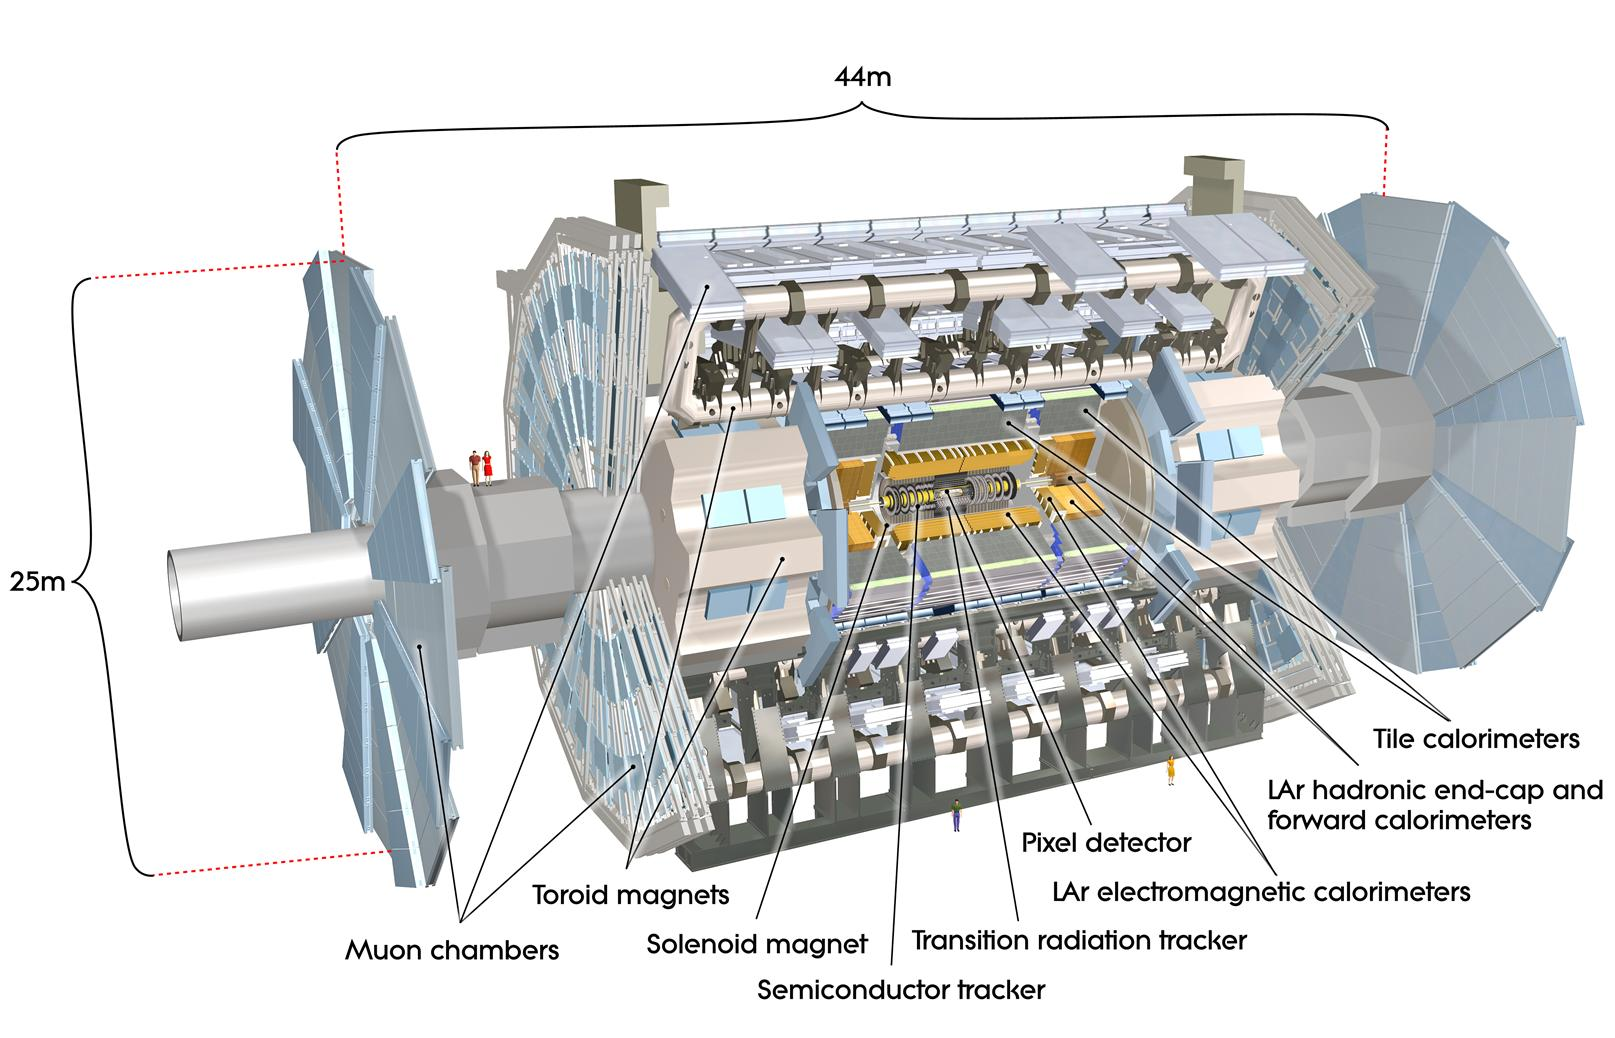
\includegraphics[width=\paperwidth]{atlas}}

 \begin{frame}
   hola
 \end{frame}
}

{\setbeamertemplate{frametitle}
{\begin{centering}\color{red}\textbf{\insertframetitle}\par\end{centering}}
\setbeamercolor{normal text}{fg=red,bg=lightgray}
%\setbeamercolor{normal text}{bg=blue}
%\setbeamercolor{normal text}{fg=red}
\begin{frame}[fragile]
\frametitle{The Title and background of This Frame.}
normal text
\begin{verbatim}
 {\begin{centering}\color{red}\textbf{\insertframetitle}\par\end{centering}}
 \setbeamercolor{normal text}{bg=blue}
 \begin{frame}[fragile]
 \frametitle{The Title of This Frame.}
 Blah, blah.
 %\end{frame}
 }
\end{verbatim}
normal text
\end{frame}
}
%%%%%%%%
{
\setbeamertemplate{blocks}[rounded][shadow=false]
\begin{frame}
  \frametitle{Get out od shadows}
  \begin{block}{hola}
    hola
  \end{block}
\end{frame}
}
%%%%%%%

\begin{frame}

\frametitle{Tic-Tac-Toe via Graphics Files}
\setbeamercovered{invisible}
\begin{center}
\multiinclude[pause=\pause,format=pdf]{game}
\end{center}
\end{frame}

\begin{frame}
\frametitle{Tic-Tac-Toe via {\tt tabular}}
\setbeamercovered{invisible}
{\Huge
\begin{center}
\begin{tabular}{c|c|c}
\onslide<9->{O} & \onslide<8->{X} & \onslide<2->{X} \\ \hline
\onslide<6->{X} & \onslide<3->{O} & \onslide<5->{O} \\ \hline
\onslide<10->{X} & \onslide<7->{O} & \onslide<4->{X}
\end{tabular}
\end{center}
}
\end{frame}

%%%%%%%%%%%%%%%%%%%%%%%%%%%%%%%%
\begin{thebibliography}{99}

\end{thebibliography}
\end{document}
